\chapter{Sensor Application}\label{sensor-application}
In this chapter the sensor application will be presented. 
Several sequence diagrams will be explained, as well as concepts needed to understand the flow of the application. 

\section{Health Sensors}
There is an ongoing discussion of when the health technology revolution will come to human bodies now that \gls{IoT} have become so popular.
By revolution, I mean sensors placed in the human body. 
Sensors that can read your blood pressure, heart rate and measure insulin levels.
Sensors that can detect whether your body is missing a substance, or if it is poisoned. 
There is no limit for what can be done.
Everything that should be measured, will be measured by sensors integrated in the human body.
But who will be able to read the \gls{data}?
Or perform instructions to the sensors/devices?
There is some major privacy issues related to this discussion, and problems that needs to be solved.

In 2011, Jerome Radcliffe discovered that his insulin pump easily could be hacked~\cite{radcliffe2011hacking}.
Basically the pump would take instructions from anyone and do anything, with no questions asked. 
This is a worst case scenario when it comes to hacking medical devices attached to a human.

For this matter I propose a \gls{HSS} that is built upon \gls{NDN} with \gls{IBC} ensuring a secure and locked environment.
First, let me introduce you to The Stig. 
He has developed diabetes and he does not want to manually monitor his glucose levels and adjust the insulin pump every meal. 
He has injected a \gls{CGM} to monitor his glucose levels and report to the insulin pump, automatically.
In addition to his diabetes, he has a heart disease which forces him to monitor his heart rate at any given time. 
In~\autoref{fig:health-sensor-system} we can see The Stig with all his sensors and devices. 
The \gls{CGM} reports periodically to the insulin pump, and all sensors reports to The Stig's mobile so that The Stig can watch what is going on.

\begin{figure}[ht]
  \centering
  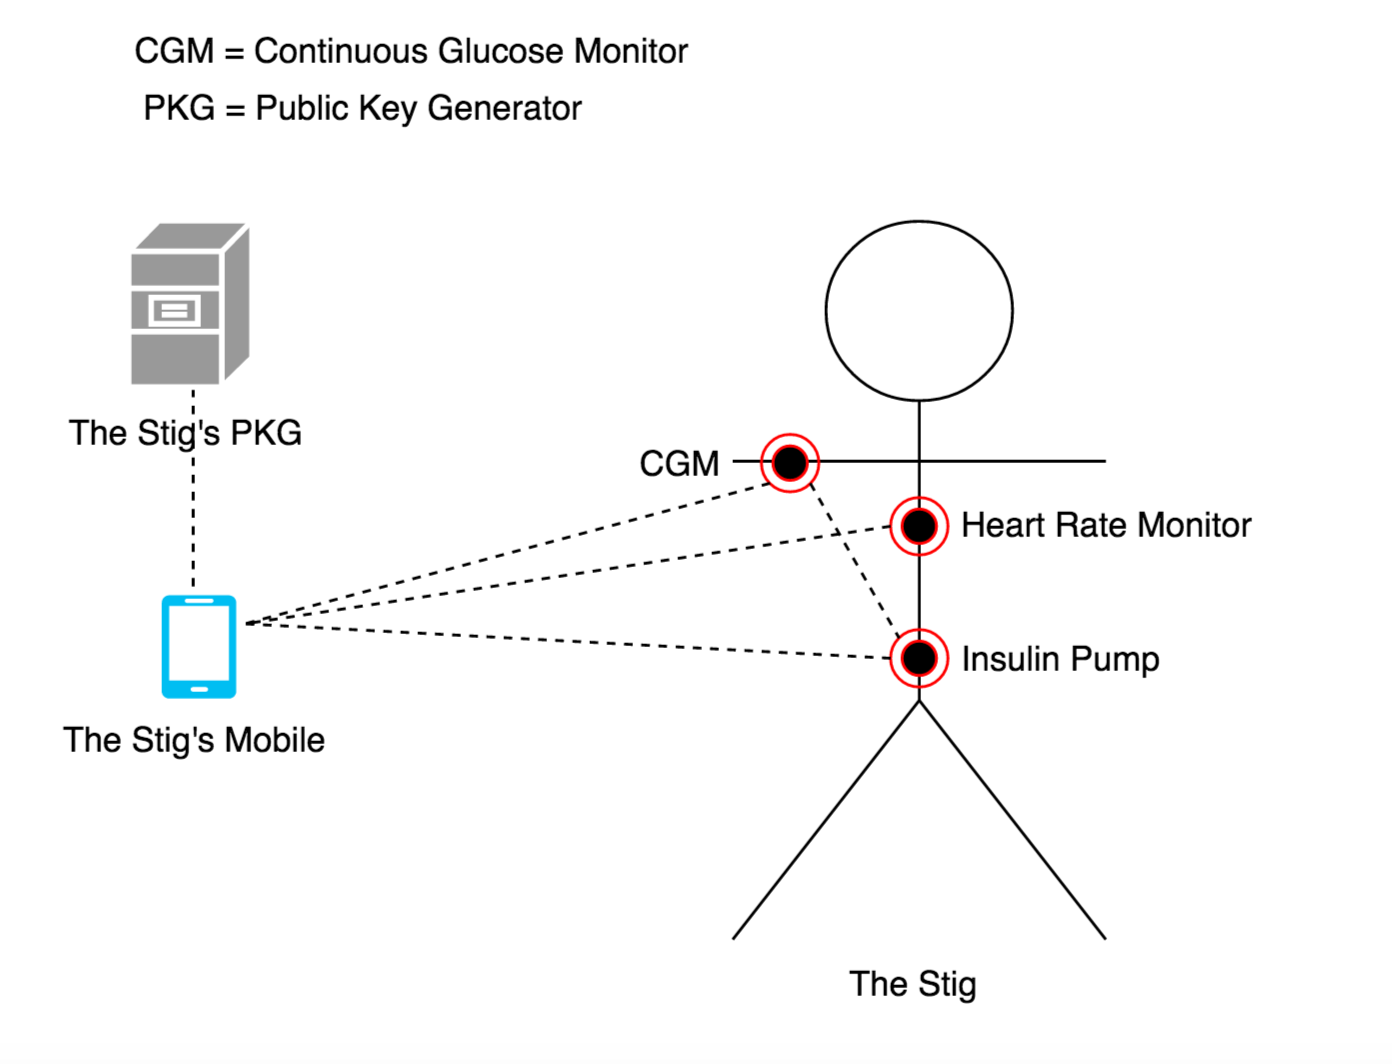
\includegraphics[width=1\textwidth]{health-sensor-system.png}
  \caption{Health Sensor System}
  \label{fig:health-sensor-system}
\end{figure}

\section{Health Sensor System}\label{hss}
To have a secure system, it needs to be established trust between the sensors and the devices.
There need to be integrity controls, confidentiality protection and access control. 
In the following sections, I will describe the protocols suggested for achieving the mentioned goals.

\subsection{Rendezvous Authentication}\label{rendezvous_authentication}
One of the best solutions for authentication of an identity in cryptography is rendezvous authentication, the concept of meeting face-to-face for authenticating who you are talking to. 
Most cases in \gls{IoT} we have the advantage of identifying devices in a physical manner.
This means that it is possible to authenticate devices, such as sensors. 
Typically, this kind of authentication will rely on 1) manually inspection and 2) digital connection, e.g. through \gls{NFC}.
In the proposed system, I assume that this type of authentication is achieved in a secure manner and do not discuss how this should be done.

Also there is the concept of human-computer authentication~\cite{DBLP:journals/iacr/GilbertRS05, DBLP:conf/crypto/JuelsW05, DBLP:conf/percom/Weis05}.
This authentication method uses a shared secret before authentication. 

\subsection{System Initialization Phase}

\subsection{Device Registration Phase}\label{init}
The goal for the initialization protocol is to achieve a secure one-round secret key exchange.
For the protocol to be secure, there are several issues that need to be addressed. 
The response message containing the secret key has to be 1) encrypted. 
This can be achieved by using asymmetric encryption on a \gls{CEK} which is used to do symmetric encryption on the secret key.
The response message has to be 2) signed by the \gls{PKG} for integrity and authenticity reasons.
For it to make sense applying 3) a nonce for replay protection, the communication between the device and the \gls{PKG} has to be unique of some kind.
This implies that the device has to authenticate itself in a way that an adversary cannot do, e.g. a shared secret.
This secret can for instance be a hardware implemented secret in the device that the user reads (from the package) and authenticates manually at the \gls{PKG} before the initialization.
% This leads to 4) mutual authentication. 

When The Stig is setting up his \gls{HSS}, first he wants to configure the \gls{PKG}. 
Any type of computer can play the role of the \gls{PKG} and The Stig has chosen his home server, from now ``the PKG''.
The \gls{PKG} creates two key pairs that is used to do \gls{IBE} and \gls{IBS}.
Second, he wants his mobile device, from now ``the mobile'', to be a part of the \gls{PKG}s trust domain, and further add all of the other devices and sensors, from now ``device(s)''.

In~\autoref{fig:init_ibe_1} the device plays the role as the mobile. 
The \gls{ID} of every device is a part of the \gls{name}.
A device register the prefix \path{/ndn/no/ntnu/<device>/<resource>} and hence its \gls{ID} is \path{/ndn/no/ntnu/<device>}.
To be able to communicate securely under initialization, the device have to create a key pair, \gls{TMPK} and \gls{TMSK}, and then extract a temporary secret key for its \gls{ID}. 
At first, the device has to act as a key generator for itself to ensure that the \gls{receiver} (i.e. the \gls{PKG}) can encrypt the extracted \gls{SK}.
The trust between the device and the real \gls{PKG} is based on the concept explained in~\autoref{rendezvous_authentication}.
The device sends an \gls{interest} appending the \gls{TMPK} and the \gls{ID} to the \gls{PKG} asking to join the \gls{PKG}s trust domain.
The \gls{PKG} encrypts a \gls{CEK} with the \gls{TMPK} and the \gls{ID} received from the device. 
The \gls{PKG} extracts the secret key for the device (this will be the key belonging to the \gls{PKG}s trust domain) and uses the \gls{CEK} to do symmetric \gls{AES} encryption on the secret key. 
The \gls{data} packet response to the initialization \gls{interest} will contain the identity-based encrypted \gls{CEK}, the symmetric encrypted secret key and the \gls{PKG}s \gls{MPK}.
To finish the initialization protocol, the device decrypts the \gls{CEK}, throws away the temporary keys, and finally decrypts the secret key.
The device has established a trust with its \gls{PKG} and can verify other devices in this domain. 

\begin{figure}[H]
  \centering
  \begin{tikzpicture}[node distance=6cm,auto,>=stealth']
      \node[] (server) {pkg};
      \node[left = of server] (client) {device};
      \node[below of=server, node distance=9cm] (server_ground) {};
      \node[below of=client, node distance=9cm] (client_ground) {};
      %
      \draw (client) -- (client_ground);
      \draw (server) -- (server_ground);
      
      \draw ($(client)!0.10!(client_ground)$) -- node[above,scale=0.8,right]{ID\textsubscript{d}, tk} ($(client)!0.10!(client_ground)$);
      \draw ($(server)!0.10!(server_ground)$) -- node[above,scale=0.8,right]{(msk, mpk), (ID\textsubscript{pkg}, sk\textsubscript{pkg})} ($(server)!0.10!(server_ground)$);
      
      \draw[->] ($(client)!0.25!(client_ground)$) -- node[above,scale=0.8,midway]{ID\textsubscript{d} || tk} ($(server)!0.25!(server_ground)$);
      \draw[<-] ($(client)!0.35!(client_ground)$) -- node[above,scale=0.8,midway]{ID\textsubscript{pkg} || mpk} ($(server)!0.35!(server_ground)$);
      \draw ($(server)!0.50!(server_ground)$) -- node[above,scale=0.8,right]{Admin manually approves ID\textsubscript{d}} ($(server)!0.50!(server_ground)$);

      \draw[->] ($(client)!0.55!(client_ground)$) -- node[above,scale=0.8,midway]{Interest: AES\_Enc\textsubscript{tk}[ID\textsubscript{d} || nonce]} ($(server)!0.55!(server_ground)$);
      \draw ($(server)!0.60!(server_ground)$) -- node[above,scale=0.8,right]{ID\textsubscript{d}, nonce = AES\_Dec\textsubscript{tk}[ID\textsubscript{d} || nonce]} ($(server)!0.60!(server_ground)$);
      \draw ($(server)!0.65!(server_ground)$) -- node[above,scale=0.8,right]{sk = Extract(mpk || msk || ID\textsubscript{d})} ($(server)!0.65!(server_ground)$);
      \draw ($(server)!0.70!(server_ground)$) -- node[above,scale=0.8,right]{c = AES\_Enc\textsubscript{tk}[sk || nonce]} ($(server)!0.70!(server_ground)$);

      \draw[<-] ($(client)!0.75!(client_ground)$) -- node[above,scale=0.8,midway]{Data: Sign(mpk || sk\textsubscript{pkg} || c)} ($(server)!0.75!(server_ground)$);
      \draw ($(client)!0.85!(client_ground)$) -- node[above,scale=0.8,right]{Verify(mpk || ID\textsubscript{pkg} || c || s)} ($(client)!0.85!(client_ground)$);
      \draw ($(client)!0.90!(client_ground)$) -- node[above,scale=0.8,right]{sk, nonce = AES\_Dec\textsubscript{tk}[c]} ($(client)!0.90!(client_ground)$);
      \draw ($(client)!0.95!(client_ground)$) -- node[above,scale=0.8,right]{mpk} ($(client)!0.95!(client_ground)$);
  \end{tikzpicture}
  \caption{Device Registration. 
  The first two messages are exchanged through e.g. NFC (\autoref{rendezvous_authentication}), and thus are protected against any adversaries outside the range of the NFC signal. 
  At first the Device generates a temporary random key \texttt{tk} and sends this key and its ID to the PKG. 
  The PKG responds with its ID and a admin user have to approve the requesting device.
  When approved, the device sends a Init Interest and receives a response with the secret key corresponding to its ID.
  }
  \label{fig:init_ibe_1}
\end{figure}


% \begin{figure}[ht]
%   \centering
%   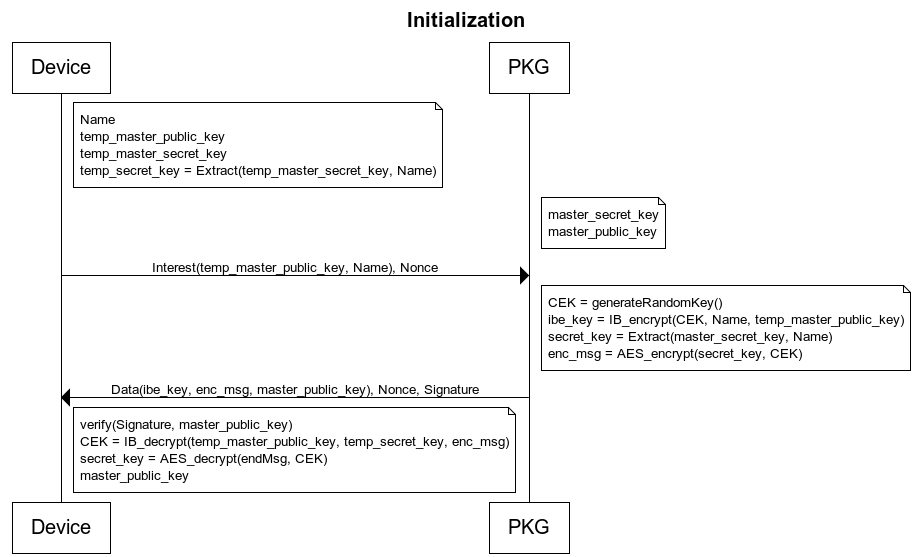
\includegraphics[width=1\textwidth]{Initialization.png}
%   \caption{Initialization IBE}
%   \label{fig:init_ibe_1}
% \end{figure}

Now that the mobile is authenticated, devices can connect to the mobile through e.g. \gls{NFC} for initialization.
This results in a rendezvous authentication between the device and the mobile, and if the mobile is given the authorities to perform initialization (\autoref{access_control}), the new device can join the \gls{PKG}s trust domain.

\subsubsection{Security Analysis}

\textit{Authenticity}.

\textit{Integrity}.

\textit{Confidentiality}. Key and data confidentiality.

\textit{Replay}.

\subsection{Deployment Phase}\label{data_pull}
The goal for this protocol is to achieve a secure one-round \gls{data} pull with authorization and integrity.
For the protocol to work and the \gls{data} pull to be successful, 1) both devices has to belong to the same trust domain (i.e. has initialized with the same \gls{PKG}) and 2) the requester has to have granted access rights for the resource requested.

As illustrated in~\autoref{fig:health-sensor-system}, the device has joined the \gls{PKG}s trust domain and is ready to communicate with other devices.
This flow is illustrated in~\autoref{fig:data_pull_ibe}.
First the requester has to express an \gls{interest} to the target device asking for a specific resource. 
The requester signs the \gls{interest} and appends it to the content \gls{name}.
The \gls{receiver} checks whether the requester has access rights to the requested resource and verifies that the requester is a part of the same trust domain.
If the \gls{receiver} is authorized, the \gls{receiver} responds with the \gls{data} containing the resource. 
The \gls{receiver} will also do a symmetric encryption on the sensor \gls{data} and do a asymmetric encryption on the \gls{CEK} with the requester's \gls{ID}.
This step is only performed if \gls{data} confidentiality is needed. 
Then the \gls{data} packet is signed and sent.
Finally the requester receives the \gls{data}, verifies the signature and decrypts the sensor \gls{data}.

\begin{figure}[H]
  \centering
  \begin{tikzpicture}[node distance=4.5cm,auto,>=stealth']
      \node[] (server) {PKG};
      \node[left = of server] (client_1) {Device};
      \node[left = of client_1] (client_0) {Mobile};
      \node[below of=server, node distance=8cm] (server_ground) {};
      \node[below of=client_0, node distance=8cm] (client_0_ground) {};
      \node[below of=client_1, node distance=8cm] (client_1_ground) {};
      %
      
      \draw (server) -- (server_ground);
      \draw (client_0) -- (client_0_ground);
      \draw (client_1) -- (client_1_ground);
      
      \draw ($(client_0)!0.10!(client_0_ground)$) 
      -- node[above,scale=0.8,right]{(ID\textsubscript{m}, sk\textsubscript{m}, mpk)} 
      ($(client_0)!0.10!(client_0_ground)$);
      \draw ($(client_1)!0.10!(client_1_ground)$) 
      -- node[above,scale=0.8,right]{(ID\textsubscript{d}, sk\textsubscript{d}, mpk)} 
      ($(client_1)!0.10!(client_1_ground)$);
      \draw ($(server)!0.10!(server_ground)$) 
      -- node[above,scale=0.8,left]{(msk, mpk)} 
      ($(server)!0.10!(server_ground)$);


      \draw ($(client_0)!0.15!(client_0_ground)$) 
      -- node[above,scale=0.8,right]{msg\textsubscript{1} = (ID\textsubscript{d} || nonce || request)} 
      ($(client_0)!0.15!(client_0_ground)$);
      \draw[->] ($(client_0)!0.30!(client_0_ground)$) 
      -- node[above,scale=0.8,midway]{Interest: Sign(mpk || ID\textsubscript{m} || msg\textsubscript{1})} 
      ($(client_1)!0.30!(client_1_ground)$);
      \draw ($(client_1)!0.35!(client_1_ground)$) 
      -- node[above,scale=0.8,right]{Verify(mpk || ID\textsubscript{m} || msg\textsubscript{1} || sign)} 
      ($(client_1)!0.35!(client_1_ground)$);
      \draw ($(client_1)!0.40!(client_1_ground)$) 
      -- node[above,scale=0.8,right]{AccesControl(ID\textsubscript{m}, request)} 
      ($(client_1)!0.40!(client_1_ground)$);
      \draw ($(client_1)!0.45!(client_1_ground)$) 
      -- node[above,scale=0.8,right]{c\_cek = Encrypt(mpk || ID\textsubscript{d} || cek)} 
      ($(client_1)!0.45!(client_1_ground)$);
      \draw ($(client_1)!0.50!(client_1_ground)$) 
      -- node[above,scale=0.8,right]{c = AES\_Enc\textsubscript{cek}(data || nonce)} 
      ($(client_1)!0.50!(client_1_ground)$);
      \draw ($(client_1)!0.55!(client_1_ground)$) 
      -- node[above,scale=0.8,right]{msg\textsubscript{2} = (c\_cek || c)} 
      ($(client_1)!0.55!(client_1_ground)$);
      \draw[<-] ($(client_0)!0.60!(client_0_ground)$) 
      -- node[above,scale=0.8,midway]{Data: Sign(mpk || ID\textsubscript{m} || msg\textsubscript{2})} 
      ($(client_1)!0.60!(client_1_ground)$);

      \draw ($(client_0)!0.70!(client_0_ground)$) 
      -- node[above,scale=0.8,right]{Verify(mpk || ID\textsubscript{d} || msg\textsubscript{2} || sign)} 
      ($(client_0)!0.70!(client_0_ground)$);
      \draw ($(client_0)!0.75!(client_0_ground)$) 
      -- node[above,scale=0.8,right]{cek = Decrypt(mpk || sk\textsubscript{d} || c\_cek)}
      ($(client_0)!0.75!(client_0_ground)$);
      \draw ($(client_0)!0.80!(client_0_ground)$) 
      -- node[above,scale=0.8,right]{data, nonce = AES\_Dec\textsubscript{cek}(c)} 
      ($(client_0)!0.80!(client_0_ground)$);
  \end{tikzpicture}
  \caption{Data pull under deployment. 
  The mobile sends a Sensor Interest to the device. 
  The Interest is signed with the mobile's SK and verified at the device. 
  The device checks whether the mobile has a valid capability for the requested resource and encrypts the data if granted.
  The Data response is signed with the device's SK.
  The mobile receives the data after decryption of the content encryption key (cek) and the cipher (c).}
  \label{fig:data_pull_ibe}
\end{figure}

% \begin{figure}[ht]
%   \centering
%   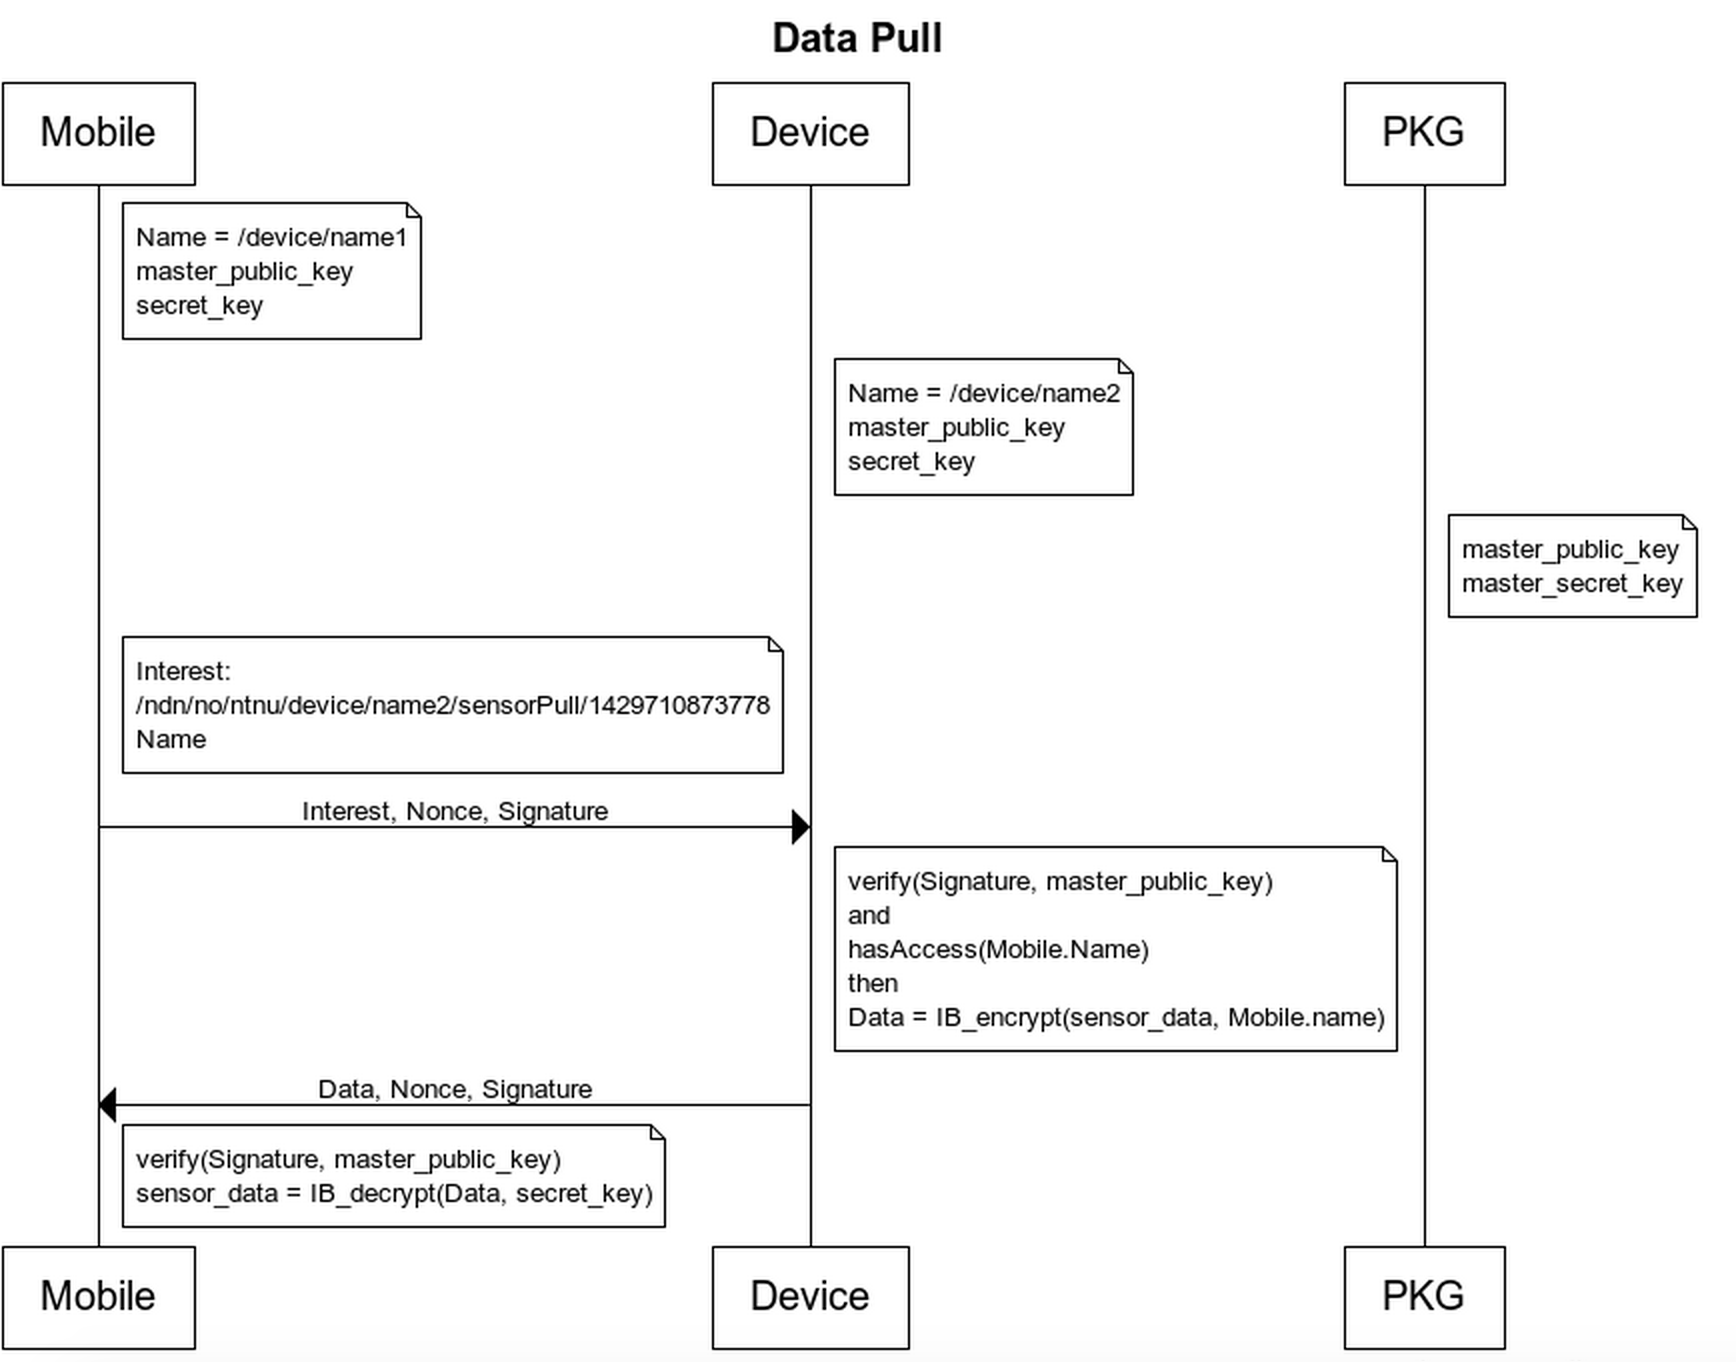
\includegraphics[width=1\textwidth]{DataPull.png}
%   \caption{Mobile performing a data pull from a device in the network.}
%   \label{fig:data_pull_ibe}
% \end{figure}

\subsubsection{Security Analysis}

\textit{Authenticity}.

\textit{Integrity}.

\textit{Confidentiality}. Key and data confidentiality.

\textit{Replay}.

\subsection{Key Distribution using File Synchronization Module}

The Stig wants to have full control over the devices that are a part of the trust domain, and be able to remove a device if necessary.
Each device should have an updated list of all public keys, i.e. every devices' \gls{ID}.
The distribution of this list can easily be achieved by using the \gls{FSM} (\autoref{file-sync} \& \autoref{key-distribution}).
The \gls{PKG} will be the distributor in this synchronization and each device will be a subscriber.


\section{Security Analysis}
In this section the security of the protocols presented in~\autoref{init} and ~\autoref{data_pull} will be proven.
\todo{!!}
Security analysis code in~\autoref{apx:scyther-analysis}

\subsection{Threat Model}
Threats that I find relevant for the \gls{HSS} can be catigorized into three main categories: threats to privacy, threats to availability and threats to control.
I assume the following threat model:
\begin{enumerate}
  \item An adversary might try to eavesdrop information (privacy).
  \item An adversary might try to send bogus commands, e.g. injection, replay and \gls{MITM} (control).
  \item Jamming, node compromise (such as theft of mobile) and \gls{DoS} (availability).
\end{enumerate}

I assume that the \gls{PKG} cannot be compromised by any adversary, and thus the \gls{MSK} will always be hidden from any adversaries. 
However, it is extremely important that the machine which plays the role of the \gls{PKG} is secured in a physical matter, as well as remote secureness. 
The \gls{PKG} is the single point of failure in the whole system.

An idea introduced by Aaditeshwar Seth and Srinivasan Keshav in~\cite[Section 5.4]{Seth:2005:PSD:1897159.1897165} is to avoid storing the \gls{SK}s in devices that is more likely to be lost or stolen, e.g. a mobile.
Using \gls{HIBC}, one can extend the key hierarchy by another level that is time-based.
These time-based keys can then be downloaded to the mobile on a daily basis, hence the time the mobile will be compromised is reduced.

\subsection{Access Control}\label{access_control}
Since the ID\textsubscript{device} is appended to the \gls{interest} and the \gls{interest} is signed by the corresponding SK\textsubscript{device}, the \gls{ID} of the device can easily be authenticated. 
When a device retrieves an \gls{interest} for its sensor \gls{data}, there should be an authorization mechanism. 
One can argue that once a device has been authenticated in the \gls{PKG}s trust domain, everyone in the domain can be sure that the device will not abuse the information or functionalities available. 
However, due to scalability this is not a secure way to handle access control. 
If a device does not need a privilege, it does not need it.
Hence it should not have it. 
That is the least privilege access principle, which is default in Capability Based Approach to \gls{IoT} Access Control~\cite{DBLP:conf/imis/GusmeroliPR12}.
This approach has some additional benefits for the \gls{HSS}, such as

\begin{itemize}
  \item delegation support - 
  A device can grant access rights to other devices, as well as granting the right to further delegate these rights to a third device.
  \item capability revocation - 
  If the \gls{PKG} have granted delegation rights to a mobile, and the mobile is not found trustworthy after a while, the capabilities issued by the mobile can easily be revoked.
  \item information granularity - 
  Specific resources from a device can be granted access to in different granularity.
\end{itemize}

Another solution can be an \gls{ACL} based approach equivalent to what Wentao Shang et al. did in~\cite{DBLP:journals/network/ShangDMBZ14}.

\subsection{Confidentiality}
The confidentiality is achieved by doing asymmetric encryption on a \gls{CEK} that is used for symmetric encryption on the content.
As explained in the sequence diagram (\autoref{fig:data_pull_ibe}) presented in the above sections, each \gls{interest} appends the requester's ID (\autoref{eq:mapping-id-name-pk}).
Since the ID\textsubscript{requester} always is appended it can always be used to do asymmetric encryption, hence all \gls{CEK}s can be encrypted only for the requesting device, and thus the confidentiality in the system can always be achieved.

\subsection{Integrity and Authenticity}
Each device will obtain a secret key allocated by its superior \gls{PKG}, as explained in~\autoref{ibc}.
With the concept from~\autoref{rendezvous_authentication} together with the \gls{PKG}s \gls{MPK}, you can trust that the device is authorized for the \gls{PKG}s trust domain. 
Hence all signed packets can be verified by anyone with the \gls{MPK}.
In this setting, a verified signature acts as an assurance of authentication and integrity. 

Every \gls{interest} has a timestamp attached to the \gls{name} (e.g. \path{/ndn/no/ntnu/device/name2/sensorPull/1429710873778}), i.e. milliseconds from \texttt{UTC} \texttt{1970-01-01} \texttt{00:00:00}, that can be used for protection against replay attack. 

\subsection{Availability}
This is a harder problem to solve.
The network is purely wireless, hence vulnerable to jamming. 
An adversary could try to send infinite \gls{interest}s to a device with an invalid signature, hence the device may be overloaded with work and might run out of battery fast.
Therefore one should check the \gls{MPK} before doing any crypto.
This is also why I have chosen to append the MPK in the packet~\autoref{fig:sensor_interest-data}. 

\subsection{Trust Model}
For a system to be secure, cryptography together with trust is essential. 
The \gls{HSS} trust model is built upon trusting a centralized authority, typically the user's home server, rendezvous authentication and \gls{IBC}.
The fact that it runs over \gls{NDN} makes it easier to achieve security goals and usability for third party developers.

The \gls{PK} is the \gls{name} of the device, and all content published by the device will begin with this \gls{name}, hence it is easy to verify that the \gls{publisher} is the owner of the content.
To be able to verify and encrypt messages, the device need the MPK\textsubscript{PKG} and the ID of the user it wants to communicate with. 
If allowed by the PKG, the public parameters MPK\textsubscript{PKG} is public for everybody that is not a part of the trust domain. 
To be able to sign and decrypt messages the device have to be a member of the trust domain and be issued a secret key mapping to the ID\textsubscript{device}.
Each device builds its trust on other devices based on that it has been verified by an administrator that controls the \gls{PKG}.
